% =====================================================================
% sections/appendix.tex — long version only (~5-8 pages)
% =====================================================================

\section{SAR vs.\ PKK rollout disagreement}
\label{app:rollout}

The IFLS contains two independent measures of the year a village
midwife first arrived in each community: the SAR module, completed by
the facility informant, and the PKK module, completed by the village
leader. Both are recorded in waves 2--5 (PKK additionally in wave~3).
Table~\ref{tab:rollout_compare} reports diagnostic statistics on the
agreement between the two measures across the 153 communities for
which both are recorded.

\begin{table}[!htbp]
\centering
\caption{SAR vs.\ PKK rollout-year agreement.}
\label{tab:rollout_compare}
% Auto-generated by code/R/07_balance_descriptives.R
\begin{tabular}{lr}
\toprule
Metric & Value \\
\midrule
Communities total & 311.000 \\
With SAR start-year & 187.000 \\
With PKK start-year & 218.000 \\
With both & 153.000 \\
Pearson rho(SAR, PKK) &   0.021 \\
Share disagreeing (both present) &   0.830 \\
Mean |SAR - PKK| (years) &   4.350 \\
\bottomrule
\end{tabular}

\end{table}

The disagreement is severe. The Pearson correlation between the two
measures is essentially zero ($\rho = 0.02$), and the two measures
disagree on the rollout year for 83 percent of the communities for
which both are recorded. The mean absolute disagreement is over four
years. The headline analysis uses the SAR measure on the rationale
that the SAR informant (typically a facility staff member) is closer
to the operational record than the village leader, and the alternative
PKK estimates appear in column~R4 of the robustness table.

The implication of this disagreement for the headline estimates is
classical attenuation toward zero: if the true rollout year were
measured perfectly we would expect tighter point estimates and
narrower confidence intervals. The size of the attenuation cannot be
recovered without an independent benchmark. The disagreement is also a
feature of the data itself rather than a coding artifact: both
measures pass the same internal consistency checks (range, monotonic
within-village across waves) and the disagreement is not concentrated
in any one province or rollout-year bin.

\section{Callaway--Sant'Anna event-study figures}
\label{app:cs_event}

Figure~\ref{fig:cs_event_study} reports the
\textcite{callawaysantanna2021} dynamic-aggregation event-study
coefficients with 95-percent confidence intervals for the four primary
outcomes, complementing the Sun--Abraham figures in
Section~\ref{sec:results}. The qualitative patterns are similar.

\begin{figure}[!htbp]
\centering
\begin{subfigure}[t]{0.49\textwidth}
\centering
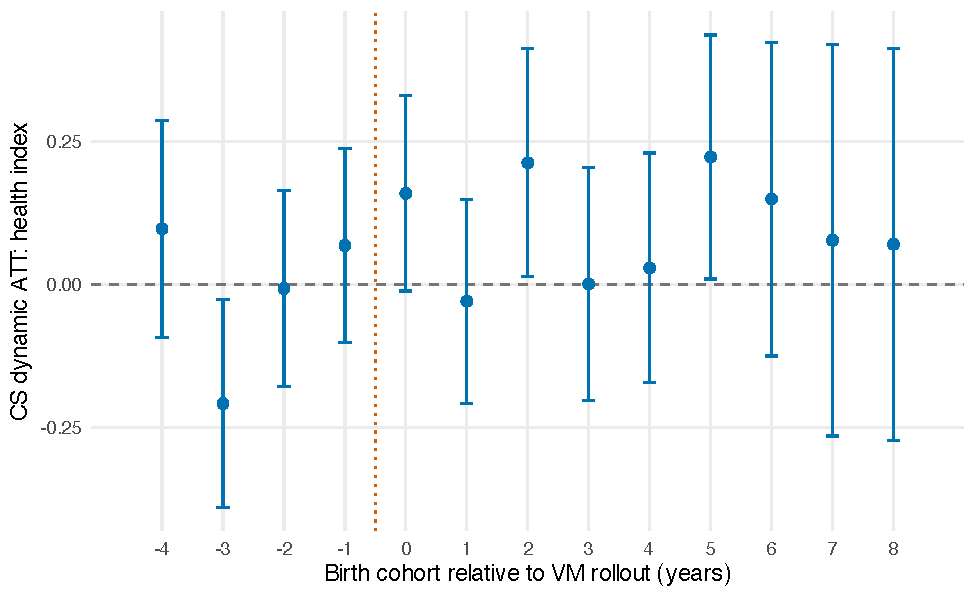
\includegraphics[width=\linewidth]{figures/event_study_CS_health_index.pdf}
\caption{Health index}
\end{subfigure}
\begin{subfigure}[t]{0.49\textwidth}
\centering
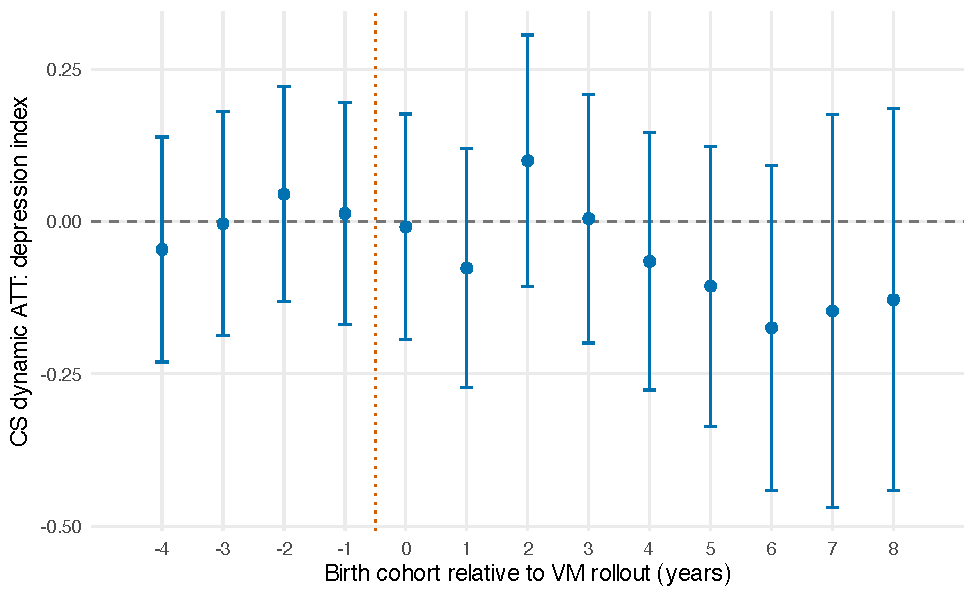
\includegraphics[width=\linewidth]{figures/event_study_CS_depression_index.pdf}
\caption{Depression index (higher = better)}
\end{subfigure}\\[1ex]
\begin{subfigure}[t]{0.49\textwidth}
\centering
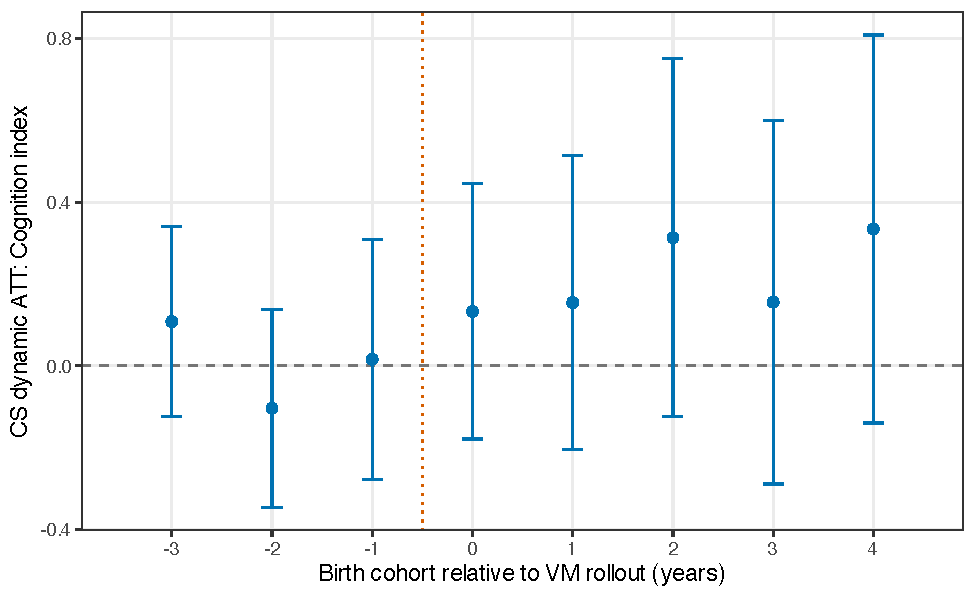
\includegraphics[width=\linewidth]{figures/event_study_CS_cognition_index.pdf}
\caption{Cognition index}
\end{subfigure}
\begin{subfigure}[t]{0.49\textwidth}
\centering
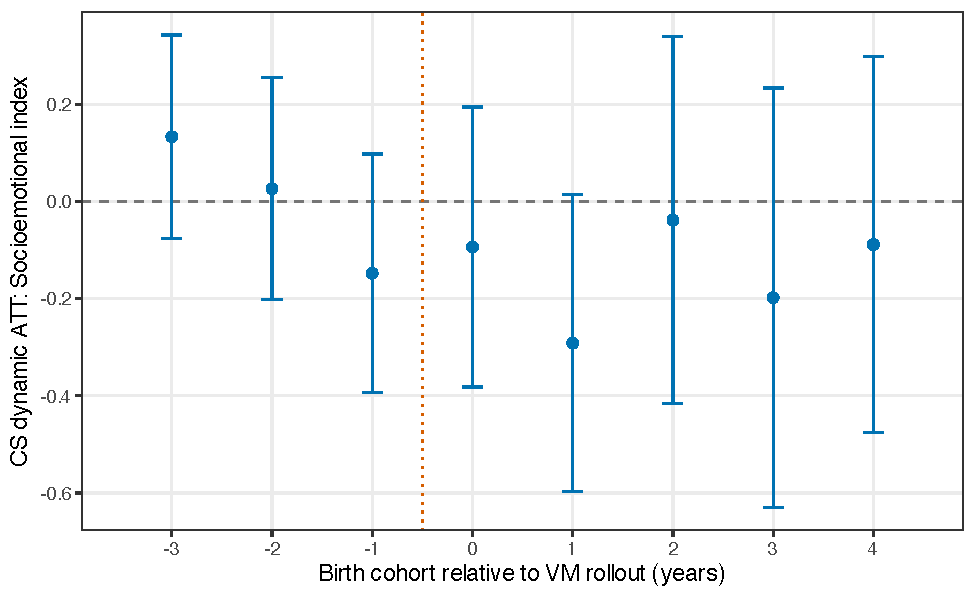
\includegraphics[width=\linewidth]{figures/event_study_CS_bigfive_index.pdf}
\caption{Big-Five index}
\end{subfigure}
\caption{Callaway--Sant'Anna dynamic-aggregation event-study
coefficients with 95\% confidence intervals.}
\label{fig:cs_event_study}
\end{figure}

\section{Event-study coefficient tables}
\label{app:event_tables}

Tables~\ref{tab:es_health} through~\ref{tab:es_bigfive} report the
event-time coefficients underlying the Sun--Abraham figures in
Section~\ref{sec:results}.

\begin{table}[!htbp]
\centering
\caption{Sun--Abraham event-study coefficients: health index.}
\label{tab:es_health}
% Auto-generated by code/R/09_event_study.R — health_index
\begin{tabular}{rccc}
\toprule
Event time & Estimate & SE & 95\% CI \\
\midrule
-4 & 0.321 & 70.179 & [-137.230, 137.872] \\
-3 & 0.015 & 0.135 & [-0.249, 0.280] \\
-2 & -0.199 & 0.152 & [-0.496, 0.099] \\
-1 & 0.000 & 0.000 & [0.000, 0.000] \\
0 & 0.408 & 0.166 & [0.083, 0.733] \\
1 & 0.199 & 154.713 & [-303.039, 303.437] \\
2 & 0.297 & 0.211 & [-0.116, 0.709] \\
3 & 0.291 & 0.265 & [-0.228, 0.810] \\
4 & -0.153 & 0.258 & [-0.659, 0.353] \\
5 & 1.209 & 0.293 & [0.635, 1.784] \\
6 & -0.214 & 0.444 & [-1.084, 0.656] \\
7 & 0.004 & 0.402 & [-0.784, 0.791] \\
8 & 0.000 & 0.000 & [0.000, 0.000] \\
\bottomrule
\end{tabular}

\end{table}

\begin{table}[!htbp]
\centering
\caption{Sun--Abraham event-study coefficients: cognition index.}
\label{tab:es_cognition}
% Auto-generated by code/R/09_event_study.R — cognition_index
\begin{tabular}{rccc}
\toprule
Event time & Estimate & SE & 95\% CI \\
\midrule
-4 & 1.586 & 29.429 & [-56.095, 59.266] \\
-3 & 0.369 & 0.134 & [0.106, 0.632] \\
-2 & 0.169 & 0.168 & [-0.161, 0.498] \\
-1 & 0.000 & 0.000 & [0.000, 0.000] \\
0 & -0.133 & 0.151 & [-0.428, 0.163] \\
1 & 4.455 & 95.690 & [-183.097, 192.007] \\
2 & 0.148 & 0.216 & [-0.275, 0.571] \\
3 & 0.082 & 0.239 & [-0.385, 0.550] \\
4 & -0.020 & 0.227 & [-0.465, 0.425] \\
5 & -2.056 & 0.275 & [-2.595, -1.516] \\
6 & -0.705 & 0.656 & [-1.990, 0.580] \\
7 & -0.625 & 0.299 & [-1.212, -0.038] \\
8 & 0.000 & 0.000 & [0.000, 0.000] \\
\bottomrule
\end{tabular}

\end{table}

\begin{table}[!htbp]
\centering
\caption{Sun--Abraham event-study coefficients: depression index.}
\label{tab:es_depression}
% Auto-generated by code/R/09_event_study.R — depression_index
\begin{tabular}{rccc}
\toprule
Event time & Estimate & SE & 95\% CI \\
\midrule
-4 & -0.205 & 1118.283 & [-2192.039, 2191.629] \\
-3 & -0.385 & 767.397 & [-1504.483, 1503.712] \\
-2 & -0.258 & 0.150 & [-0.553, 0.037] \\
-1 & 0.000 & 0.000 & [0.000, 0.000] \\
0 & 0.267 & 0.176 & [-0.079, 0.613] \\
1 & -0.095 & 5635.626 & [-11045.923, 11045.732] \\
2 & 0.168 & 360.256 & [-705.934, 706.271] \\
3 & -0.228 & 0.230 & [-0.679, 0.223] \\
4 & 0.256 & 0.212 & [-0.159, 0.672] \\
5 & -2.638 & 0.561 & [-3.738, -1.538] \\
6 & -0.665 & 0.460 & [-1.567, 0.236] \\
7 & 0.865 & 0.241 & [0.393, 1.338] \\
8 & 0.000 & 0.000 & [0.000, 0.000] \\
\bottomrule
\end{tabular}

\end{table}

\begin{table}[!htbp]
\centering
\caption{Sun--Abraham event-study coefficients: Big-Five index.}
\label{tab:es_bigfive}
% Auto-generated by code/R/09_event_study.R — bigfive_index
\begin{tabular}{rccc}
\toprule
Event time & Estimate & SE & 95\% CI \\
\midrule
-4 & -0.229 & 1541.149 & [-3020.881, 3020.423] \\
-3 & -0.016 & 1057.808 & [-2073.319, 2073.288] \\
-2 & -0.108 & 0.183 & [-0.467, 0.252] \\
-1 & 0.000 & 0.000 & [0.000, 0.000] \\
0 & -0.071 & 0.176 & [-0.417, 0.274] \\
1 & -0.352 & 7767.297 & [-15224.253, 15223.550] \\
2 & -0.107 & 496.537 & [-973.320, 973.105] \\
3 & -0.409 & 0.209 & [-0.818, 0.000] \\
4 & 0.166 & 0.210 & [-0.246, 0.577] \\
5 & -2.943 & 0.363 & [-3.655, -2.232] \\
6 & -0.502 & 0.790 & [-2.050, 1.047] \\
7 & -0.658 & 0.452 & [-1.544, 0.229] \\
8 & 0.000 & 0.000 & [0.000, 0.000] \\
\bottomrule
\end{tabular}

\end{table}

\section{Data pipeline}
\label{app:pipeline}

The analysis is fully reproducible from raw IFLS data. The pipeline
is implemented in twelve numbered R scripts orchestrated by
\texttt{code/R/00\_run\_all.R} and runs end-to-end in approximately
one minute on a modern laptop.

\begin{description}
\item[Stages 01--05 (data construction).]
Stage 01 reads the raw Stata files for IFLS waves 1--5 and writes
typed \texttt{.rds} caches. Stage 02 builds the individual-level birth
roster for cohorts 1984--1999, attaches mother covariates, computes
the three \texttt{commid\_birth} variants, and flags movers and
deaths. Stage 03 computes the SAR and PKK rollout years and the
SAR/PKK comparison diagnostic. Stage 04 extracts the wave-5 outcome
modules. Stage 05 merges these into the analysis frame and runs an
audit against the legacy DEPII analysis frame.

\item[Stages 06--12 (analysis).]
Stage 06 applies sample restrictions, constructs the four
\textcite{anderson2008} composite indices, and computes the
inverse-probability weights used in robustness column~R1. Stage 07
produces the balance table, the SAR/PKK diagnostic table, and the
descriptive Table~1. Stage 08 fits the main TWFE, Callaway--Sant'Anna,
and de Chaisemartin--D'Haultf{\oe}uille specifications. Stage 09
fits the Sun--Abraham event-study specification and the corresponding
CS dynamic aggregations. Stage 10 fits the within-mother
specifications and the fertility-selection check. Stage 11 fits the
remaining robustness columns. Stage 12 fits the heterogeneity
specifications and writes the in-text macros to
\texttt{paper/numbers.tex}.
\end{description}

The repository is organized so that all numerical content in the paper
flows from the pipeline: tables under \texttt{paper/tables/} are
produced by R scripts and included via \texttt{\textbackslash input};
figures under \texttt{paper/figures/} are produced by R scripts and
included via \texttt{\textbackslash includegraphics}; in-text numbers
flow through the \texttt{numbers.tex} macros. No numbers in the paper
are typed by hand.
